\documentclass[conference]{IEEEtran}

\usepackage[T1]{fontenc}
\usepackage{lmodern}
\usepackage{microtype}
\usepackage{tikz}
\usetikzlibrary{arrows.meta, positioning, fit, calc}
\usepackage{caption}

\begin{document}

\title{System Architecture for Perception-Integrated Navigation on TurtleBot 4}
\author{\IEEEauthorblockN{Quang Doan}}
\maketitle

\begin{figure}[t]
\centering
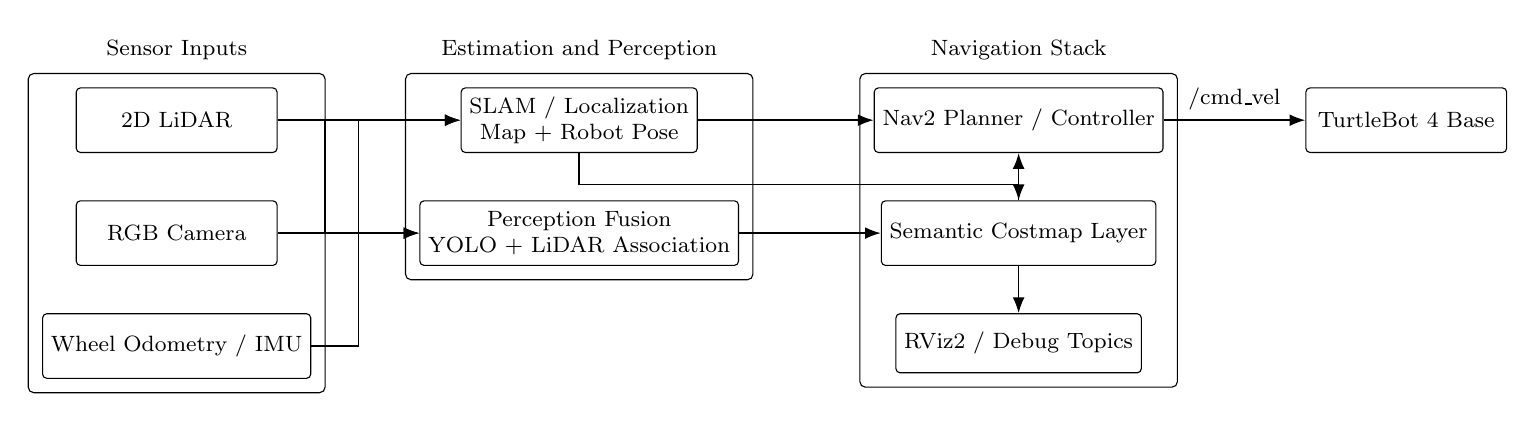
\begin{tikzpicture}[
    font=\footnotesize,
    >=Latex,
    node distance=6mm and 8mm,
    block/.style={
        draw,
        rounded corners=1.5pt,
        align=center,
        minimum width=2.55cm,
        minimum height=0.82cm,
        inner sep=3pt
    },
    smallblock/.style={
        draw,
        rounded corners=1.5pt,
        align=center,
        minimum width=2.35cm,
        minimum height=0.75cm,
        inner sep=3pt
    },
    group/.style={
        draw,
        rounded corners=2pt,
        inner sep=5pt
    },
    line/.style={
        -Latex,
        semithick
    }
]

% Inputs
\node[block] (lidar) {2D LiDAR};
\node[block, below=of lidar] (camera) {RGB Camera};
\node[block, below=of camera] (odom) {Wheel Odometry / IMU};

% Middle
\node[block, right=18mm of camera] (fusion) {Perception Fusion\\YOLO + LiDAR Association};
\node[block, above=of fusion] (slam) {SLAM / Localization\\Map + Robot Pose};

% Right
\node[block, right=18mm of fusion] (costmap) {Semantic Costmap Layer};
\node[block, above=of costmap] (planner) {Nav2 Planner / Controller};
\node[block, right=18mm of planner] (robot) {TurtleBot 4 Base};

% Bottom
\node[smallblock, below=of costmap] (viz) {RViz2 / Debug Topics};

% Arrows from sensors
\draw[line] (lidar.east) -- ++(6mm,0) |- (slam.west);
\draw[line] (lidar.east) -- ++(6mm,0) |- (fusion.west);
\draw[line] (camera.east) -- (fusion.west);
\draw[line] (odom.east) -- ++(6mm,0) |- (slam.west);

% Internal processing
\draw[line] (slam.east) -- (planner.west);
\draw[line] (fusion.east) -- (costmap.west);
\draw[line] (slam.south) -- ++(0,-4mm) -| (costmap.north);

% Costmap to planner
\draw[line] (costmap.north) -- ++(0,4mm) -| (planner.south);

% Planner to robot
\draw[line] (planner.east) -- node[above] {/cmd\_vel} (robot.west);

% Debug output
\draw[line] (costmap.south) -- (viz.north);

% Group boxes
\node[group, fit=(lidar)(camera)(odom), label=above:{\strut Sensor Inputs}] {};
\node[group, fit=(slam)(fusion), label=above:{\strut Estimation and Perception}] {};
\node[group, fit=(costmap)(planner)(viz), label=above:{\strut Navigation Stack}] {};

\end{tikzpicture}

\caption{Software architecture for a TurtleBot 4 research platform integrating LiDAR-based SLAM, learning-based perception, a semantic costmap layer, and Nav2 planning/control.}
\label{fig:system_architecture}
\end{figure}

\end{document}